% --
% spectrogram

\section{Spectral Features}\label{sec:signal_spec}
Spectral features of audio signals usually incorporate frequency information and are therefore the most intuitive form to represent them.
Often the first approach when analyzing speech signals is to visualize its spectrogram.
This allows the observation of active energy regions of certain frequency bands at consecutive time chunks and may, for example, provide hints of certain phonemes in speech signals.
Methodically, the time chunks of a spectrogram are expressed by shifting an \emph{analytic window} of time span $t_N$ on the time axis.
The time shifting of the analytic window is performed through a fixed time step, denoted as \emph{hop time} $t_{h}$.
Both time parameters $t_N$ and $t_h$ can also be presented in samples through a multiplication with the sampling frequency $f_s$, such as
\begin{equation}
  \begin{split}
    N &= t_N f_s, \\
    h &= t_h f_s.
  \end{split}
\end{equation}
Note that shifting an analytic window of sample size $N$ with hop size $h$ will create a new resolution on the time axis, referred to as \emph{frames}.
The transformation of the audio signal $x[n]$ with sample index $n$, which is contained by the analytic window of size $N$, to the frequency space, can be achieved through the Discrete Fourier Transform (DFT) defined by
\begin{equation}\label{eq:signal_spec_dtft}
  \hat{x}[k] = \sum_{n=0}^{N-1} x[n] \, e^{-j\frac{2 \pi n}{N}k},
\end{equation}
where $\hat{x}[k] \in \C$ is the transformed signal with frequency index $k$.
More conveniently, \req{signal_spec_dtft} can be written in matrix notation with the DFT operator denoted as $\mathcal{F} \in \C^{K \times N}$ with $K$ Fourier coefficients and a total number of $N$ samples of the input signal $\bm{x} \in \R^N$  as follows:
\begin{equation}\label{eq:signal_spec_dtft_matrix}
  \begin{aligned}
    \hat{\bm{x}} = \mathcal{F} \bm{x} \quad \mathrm{with} 
    \quad &\mathcal{F}[k, n] = e^{-j\frac{2 \pi n}{N} k},\\
    &k, n = (0, 1, \dots, K-1), (0, 1 \dots, N-1).
  \end{aligned}
\end{equation}
Note that $k$ and $n$ are row and column indices in the transformation matrix $\mathcal{F}$ and $\hat{\bm{x}} \in \C^K$ is the transformed signal in vector notation.

The length of the analytic window in samples $N$ is essential for the frequency resolution and the lowest frequency that can be represented.
For example, the time duration of a periodic signal with frequency $f=\SI{20}{\hertz}$ is $t=\frac{1}{f} = \SI{50}{\milli\second}$.
To represent a waveform, it is necessary to have at least a quarter of its wavelength captured.
Within this thesis, the length of the analytic window is selected to \SI{25}{\milli\second}, which is adequate for speech signals.

The \emph{hop size} $h$ in samples of the hop time $t_h$ by which the analytical window is shifted on the time axis, indicates the resolution in time and is especially important for sequential changes within the audio data.
In applications like speech processing the hop time should be selected so that the fastest pronounced phonemes and its transitions to other phonemes are captured with sufficient resolution.
Usually a hop time of $t_{h}=\SI{10}{\milli\second}$ is chosen for speech recognition tasks (also used within this thesis) but an extension to $t_{h}=\SI{20}{\milli\second}$ is also possible, as demonstrated by \cite{Peter2020}.

With the hop size $h$ in samples and $N$ the length of the analytical window, the Short-Time Fourier Transform (STFT) for discrete time signals can be defined by
\begin{equation}\label{eq:signal_spec_stft}
  \tilde{X}[k, m] = \sum_{n=0}^{N-1} x[n + m h] \, w[n] \, e^{-j\frac{2 \pi n}{N}k}, \qquad m = 0, 1, \dots, M
\end{equation}
so that $\tilde{X}[k, m] \in \C$ is the STFT of frequency coefficient $k$ and frame $m$.
Further, $n$ is the summation index, $w$ a window function, such as the \emph{Hanning} window, $h$ is the hop size, and $M$ is the maximum number of frames.
The maximum number of frames $M$ is the total number of shifts of an analytical window of size $N$ by the hop size $h$ and can therefore be determined by
\begin{equation}\label{eq:signal_spec_hop}
  M = \ceil*{\frac{\norm{\bm{x}}_0-N}{h}},
\end{equation}
where $\norm{\bm{x}}_0$ refers to the length of the signal vector $\bm{x}$.
The calculation of the STFT can be written in matrix notation if the input chunks from the shifting of the analytic window is formulated as vector
\begin{equation}
  \bm{x}_m = [x_{m h}, \dots, x_{m h+N}]^T,
\end{equation}
where each individual $\bm{x}_m \in \R^N$ can be concatenated in a matrix $X \in \R^{N \times M}$ denoted as
\begin{equation}
  X = [\bm{x}_0, \bm{x}_1, \dots, \bm{x}_M].
\end{equation}
Further, the STFT $\tilde{X} \in \C^{K \times M}$ can be conveniently written as
\begin{equation}\label{eq:signal_spec_stft_matrix}
  \tilde{X} = \mathcal{F} \diag{\bm{w}} X,
\end{equation}
where $\diag{\bm{w}}$ is a diagonal matrix of weight vectors with a realization of a window function $\bm{w} \in \R^N$ in vector notation.
The matrix $\tilde{X} \in \C^{K \times M}$ represents the whole STFT, where the rows correspond to Fourier coefficients and the columns to frames.
The used STFT parameters for this thesis are listed in \rtab{signal_spec_stft}.
% --
% stft params
\begin{table}[ht!]
\begin{center}
\caption{Parameters used for the STFT computation.}
\begin{tabular}{ M{4cm}  M{4cm}}
\toprule
\textbf{Parameter} & \textbf{Value} \\
\midrule
Sampling Frequency & \SI{16}{\kilo\hertz}\\
Analytic window size & \SI{25}{\milli\second}\\
Hop size & \SI{10}{\milli\second}\\
Window Function & Hanning\\
\bottomrule
\label{tab:signal_spec_stft}
\end{tabular}
\end{center}
\vspace{-4mm}
\end{table}
\FloatBarrier
\noindent
A spectrogram $P \in \R^{K \times M}$ is the power spectrum of the STFT $\tilde{X} \in \C^{K \times M}$ and can be defined by
\begin{equation}\label{eq:signal_spec_spec}
  P = \abs{\tilde{X}}^2.
\end{equation}
Note that $P$ consists of real values instead of complex ones.
The recorded examples transformed to a spectrogram with linear representation are shown in \rfig{signal_spec_lin_showcase}.
\begin{figure}[!ht]
  \centering
    \subfigure[left]{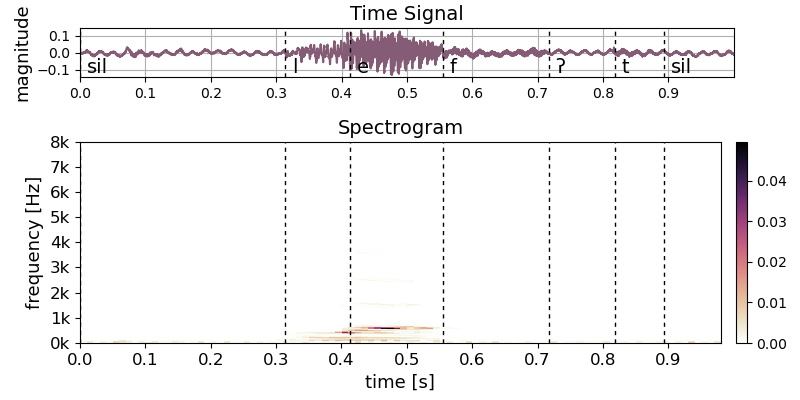
\includegraphics[width=0.45\textwidth]{./3_signal/figs/signal_spec-lin_showcase_left0.png}}
    \quad
    \subfigure[right]{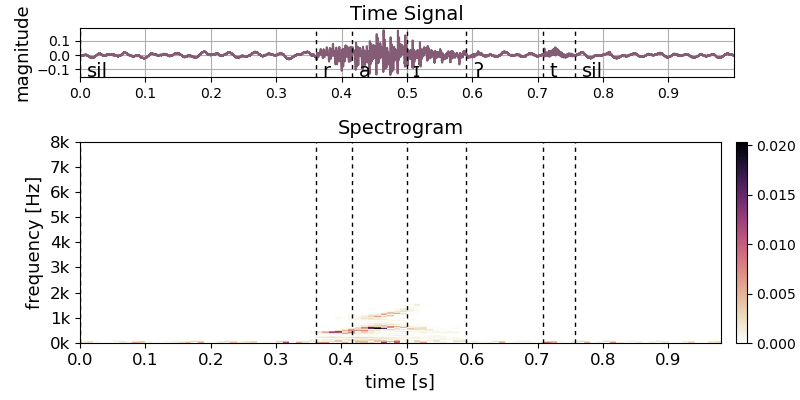
\includegraphics[width=0.45\textwidth]{./3_signal/figs/signal_spec-lin_showcase_right0.png}}
    \subfigure[up]{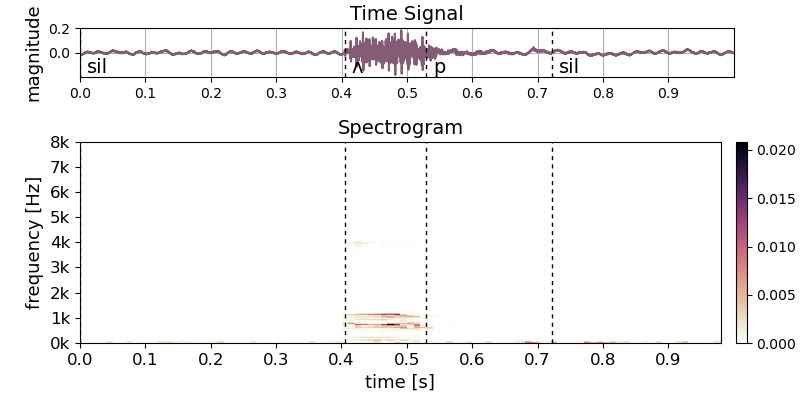
\includegraphics[width=0.45\textwidth]{./3_signal/figs/signal_spec-lin_showcase_up0.png}}
    \quad
    \subfigure[down]{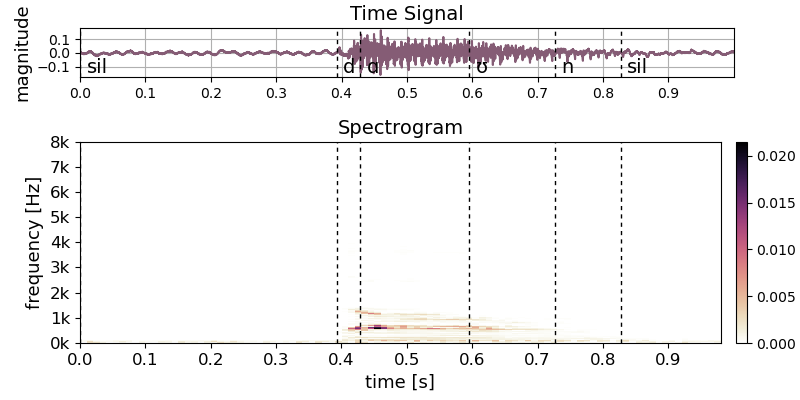
\includegraphics[width=0.45\textwidth]{./3_signal/figs/signal_spec-lin_showcase_down0.png}}
    \subfigure[go]{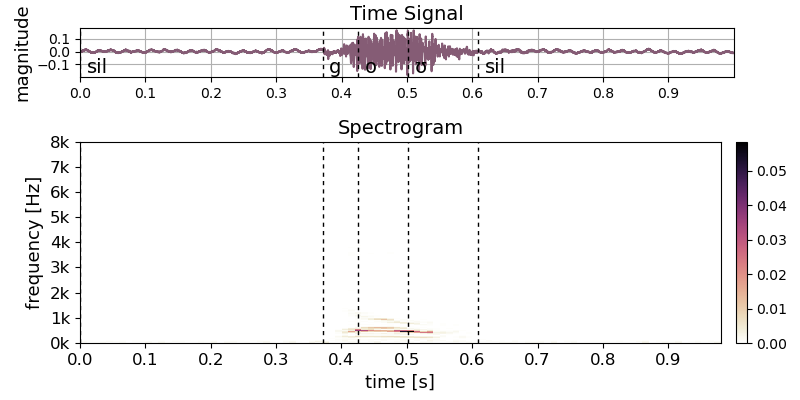
\includegraphics[width=0.45\textwidth]{./3_signal/figs/signal_spec-lin_showcase_go0.png}}
  \caption{Linear scaled spectrogram of the showcase examples.}
  \label{fig:signal_spec_lin_showcase}
\end{figure}
\FloatBarrier
\noindent
It can be observed that most of the signal's energy is located in the lower frequency regions below approximately \SI{1}{\kilo\hertz}.
To ensure that small energies are more emphasized, it is more appealing to logarithmically scale the value space of the spectrogram.
For instance, this can be achieved by the calculation of the decibel scale of the spectrogram $P_{DB} \in \R^{K \times M}$ by
\begin{equation}\label{eq:signal_spec_log}
  P_{DB} = 10 \cdot \log_{10}{P}.
\end{equation}
\rfig{signal_spec_log_showcase} visualizes the showcase examples of the logarithmically scaled spectrogram and log scaled frequency space, where it is possible to observe some interesting structures and movements in certain frequency bands over time.
\begin{figure}[!ht]
  \centering
    \subfigure[left]{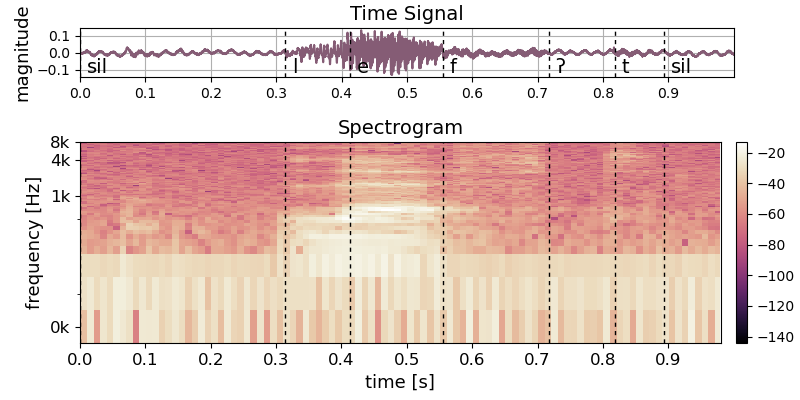
\includegraphics[width=0.45\textwidth]{./3_signal/figs/signal_spec-log_showcase_left0.png}}
    \quad
    \subfigure[right]{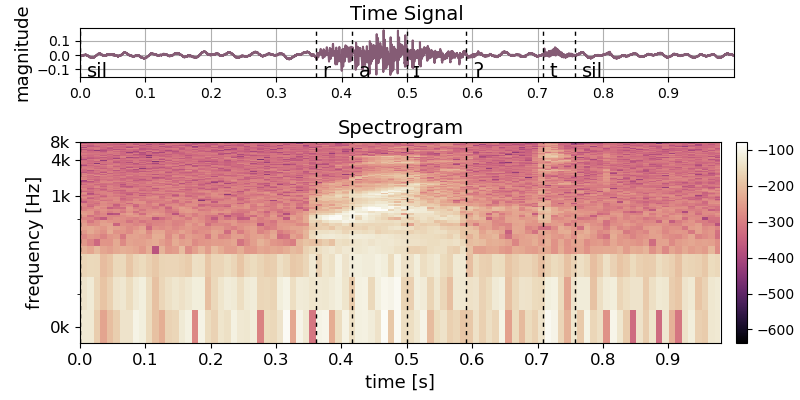
\includegraphics[width=0.45\textwidth]{./3_signal/figs/signal_spec-log_showcase_right0.png}}
    \subfigure[up]{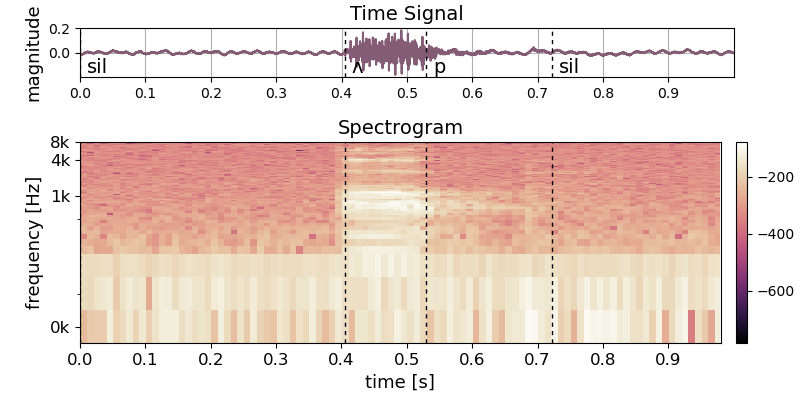
\includegraphics[width=0.45\textwidth]{./3_signal/figs/signal_spec-log_showcase_up0.png}}
    \quad
    \subfigure[down]{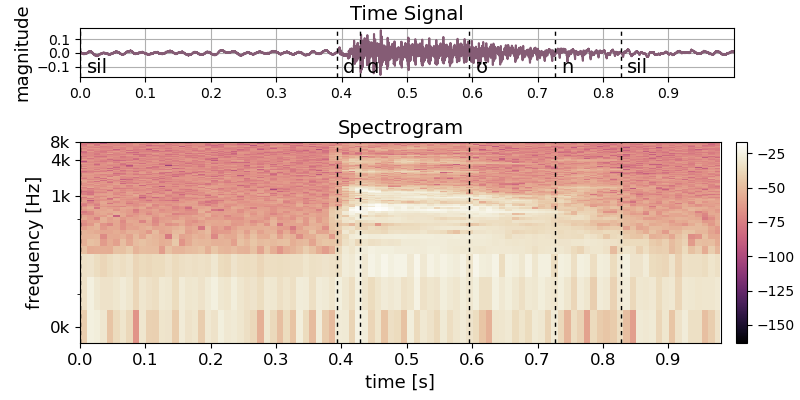
\includegraphics[width=0.45\textwidth]{./3_signal/figs/signal_spec-log_showcase_down0.png}}
    \subfigure[go]{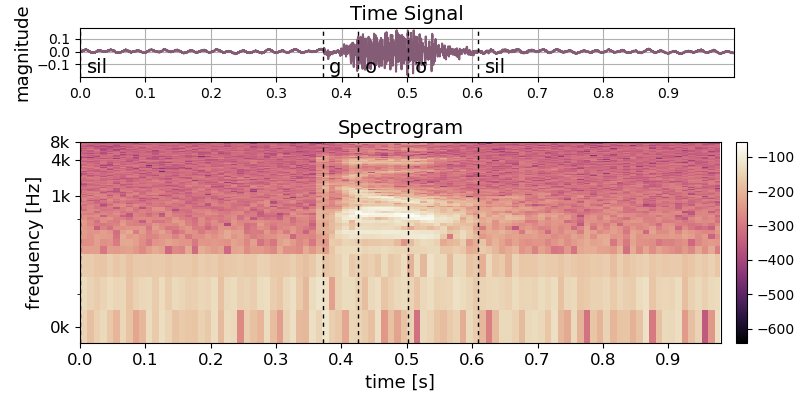
\includegraphics[width=0.45\textwidth]{./3_signal/figs/signal_spec-log_showcase_go0.png}}
  \caption{Logarithmically scaled spectrogram of the showcase examples.}
  \label{fig:signal_spec_log_showcase}
\end{figure}
\FloatBarrier
\noindent
A compression scheme, such as the MFCC explained in the next section, reduces the high dimensional frequency feature vectors of the spectrogram to more compact feature vectors.